\subsection{Exponential-Trapezoidal Discretization}
\label{sec:method:trap}
Structured SSMs are naturally defined as continuous-time dynamical systems that map input functions, $x(t) \in \mathbb{R}$,  to output functions, $y(t) \in \mathbb{R}$, for time $t > 0$.
The underlying continuous state space system is defined by a first-order ordinary differential equation (ODE) for the state $\dot{\vh}(t)$ and an algebraic equation for the output $y(t)$.
In sequence modeling, however, the data is only observed at discrete time steps, which then requires applying a \emph{discretization step} to the SSM to transform its continuous-time dynamics into a discrete recurrence.
\begin{figure}
    \vspace{-1cm}
    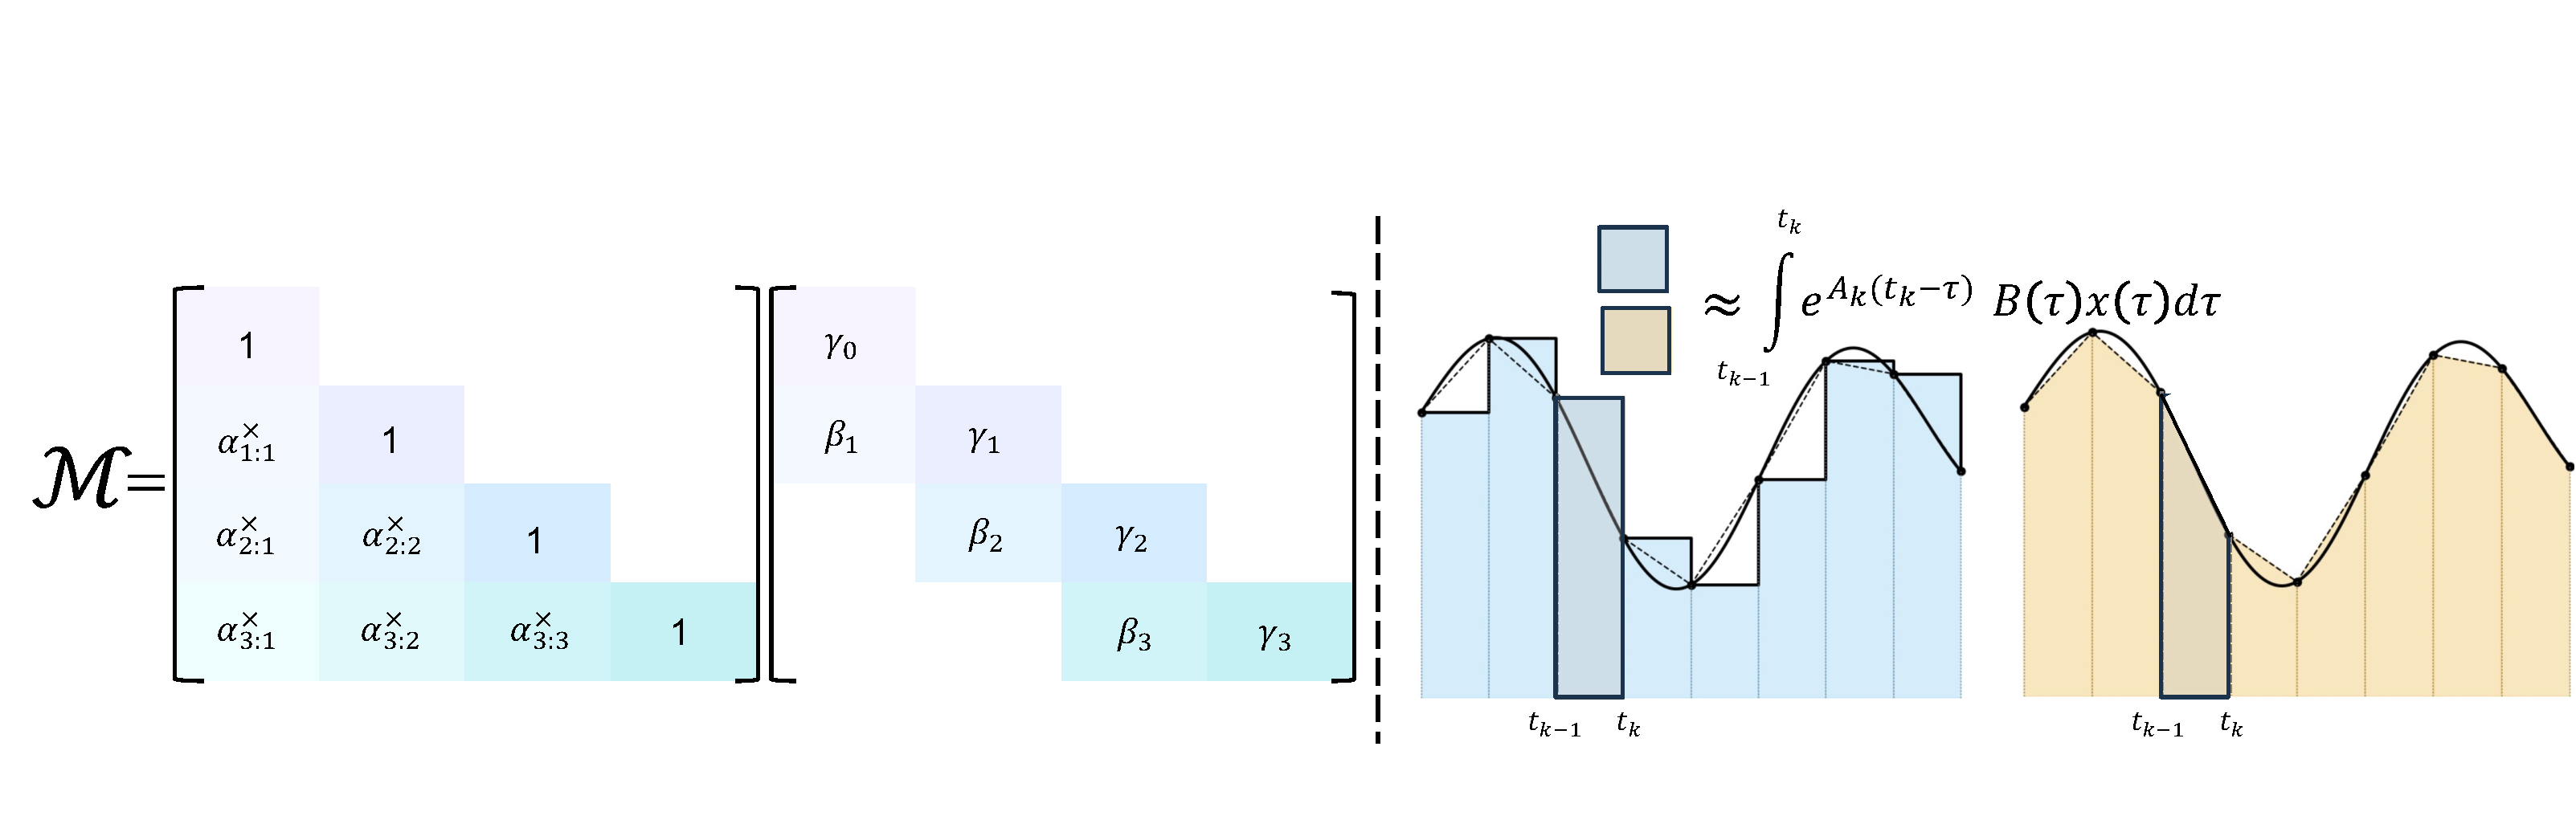
\includegraphics[width=\linewidth]{fig/trapezoid.pdf}
    \caption{\textbf{Left:} The structured mask induced by the exponential-trapezoidal rule (\Cref{sec:method:trap}) is a product of the decay and two-band convolutional mask. \textbf{Right:} Euler (hold endpoint) versus Trapezoidal (average endpoints) integral approximation.} 
    \label{fig:trap}
\end{figure}

\begin{table*}[t]
  \centering
  \small
  \renewcommand{\arraystretch}{1.2}
  \newcommand{\minitab}[2][l]{\renewcommand{\arraystretch}{1.0}\begin{tabular}[#1]{@{}#1@{}}#2\end{tabular}}
  \caption{
  Table of canonical linear-time invariant discretizations (top) and custom linear-time varying discretizations derived from our exponential-adjusted framework (bottom), along with their appearance in structured SSMs used in deep learning.
  Our theory formalizes the prior Mamba discretization as exponential-Euler and extends it with the more expressive exponential-trapezoidal method. 
  The generalized discretization framework converts a continuous SSM $\dot{\vh(t)} = \bA(t) \vh(t) + \bB(t) x(t)$ into the discrete recurrence $\vh_t = \alpha_t \vh_{t-1} + \beta_t \bB_{t-1} x_{t-1} + \gamma_t \bB_t x_t$, where various discretization methods yield different formulas for $\alpha_t, \beta_t, \gamma_t$.
  }
  \resizebox{\textwidth}{!}{
    \begin{tabular}{@{}lllll@{}}
        \toprule
        \textbf{Discretization Method} &
        $\alpha_t$ &
        $\beta_t$ &
        $\gamma_t$ &
        \textbf{Appearance} \\
        \midrule
        \textbf{Forward Euler} &
        $I + \Delta A$ &
        --- &
        $\Delta$ &
        --- \\
        \textbf{Backward Euler} &
        $(I-\Delta A)^{-1}$ &
        --- &
        $(I-\Delta A)^{-1}\,\Delta$ &
        --- \\
        \textbf{Trapezoidal} &
        $(I-\frac{\Delta}{2}A)^{-1}\,(I+\frac{\Delta}{2}A)$ &
        --- &
        $(I-\frac{\Delta}{2}A)^{-1}\,\Delta$ &
        S4 \\
        \textbf{Zero-Order Hold} &
        $\exp({\Delta A})$ &
        --- &
        $A^{-1}\,\left(\exp({\Delta A})-I\right)$ &
        \minitab{S4D, S5} \\
        \addlinespace[0.6ex]
        \midrule
        \textbf{Zero-Order Hold} &
        $\exp({\Delta_tA_t})$ &
        --- &
        $A_t^{-1}\,\left(\exp({\Delta_tA_t})-I\right)$ & 
        \\
        \textbf{Exponential-Euler} &
        $\exp({\Delta_tA_t})$ &
        --- &
        $\Delta_t$ &
        Mamba-1, -2\footnotemark \\
        \textbf{Exponential-Trapezoidal} &
        $\exp({\Delta_tA_t})$ &
        $(1-\lambda_t)\Delta_t\,\exp({\Delta_tA_t})$ &
        $\lambda_t\,\Delta_t$ &
        Mamba-3 \\
        \bottomrule
      \end{tabular}
    }
  \label{tab:discretizations}
\end{table*}
\footnotetext{While the Mamba-1 paper reports ZOH discretization, the implementation follows \url{https://github.com/state-spaces/mamba/issues/129}.}

Discretization methods are well-studied in classical control theory with several canonical formulas used in earlier SSM works in deep learning~\citep{S4,S4D,S5}.
These mechanisms were traditionally stated and applied to linear-time invariant (LTI) systems, and their derivations do not directly apply to linear-time varying (LTV) systems.
Additionally, while Mamba-1 adapted the zero-order hold (ZOH) method to LTV systems without proof, the complexity associated with selective SSMs prompted the use of an additional heuristic approximation that lacked theoretical justification and did not correspond to any established discretization technique.
In the following subsection, we formalize the previous heuristics used in current LTV SSMs through our discretization framework and utilize it to propose a more expressive discretization scheme.
\subsubsection{Overview of Exponential-Adjusted Discretization}
We introduce a simple derivation that leads to a class of new discretization methods for LTV state space models. The method can be instantiated in various ways; we show that one instantiation results in the heuristic used in Mamba-1/2, thereby theoretically justifying it (exponential-Euler). We also introduce a more powerful discretization (exponential-trapezoidal) used in Mamba-3.

The high-level intuition of our derivation originates from the closed form solution $x(t) = e^{tA}x(0)$ of a simple linear ODE $x'(t) = Ax(t)$, which discretizes to $x_{t+1} = e^{\Delta A}x_t$.
In this example, the exponential dominates the dynamics of the underlying first-order ODE, resulting in imprecise approximations when using low-order methods without significantly constraining $\Delta$.
Thus, we analyze the dynamics of the \emph{exponential-adjusted} system $e^{-At}x(t)$.
The adjusted system yields a discrete recurrent form where the state-transition and the state-input integrals are approximated separately---the state-transition integral is approximated by a right-hand approximation, i.e. $A(s) \coloneqq A(\tau_t)$ for all $s \in [\tau_{t-1},\tau_t]$, yielding,
\begin{align*}
    \vh(\tau_t) &= \underbrace{\exp\left(\int_{\tau_{t-1}}^{\tau_t}A(s)ds\right)\vh(\tau_{t-1})}_\text{via right-hand approximation} + \underbrace{\int_{\tau_{t-1}}^{\tau_t} \exp\left(\int_{\tau}^{\tau_t}A(s)ds\right)\bB(\tau)x(\tau) d\tau}_\text{via different discretization schemes},
    \\
    \vh_t &\approx \exp\left(\Delta_t A_t\right)\vh_{t-1} + \int_{\tau_{t-1}}^{\tau_t} \exp\left((\tau_t -\tau)A_t\right)\bB(\tau)x(\tau) d\tau,
\end{align*}
which serves as the foundation for further discretization techniques for the state-input integral. The full derivation is detailed in \Cref{prop:var-const}.

\paragraph{ZOH.}
The classical zero-order hold discretization method can be derived from the foundation above with a specific approximation of the right-hand side integral.
By treating $A_t, \bB(\tau), x(\tau)$ as constants over the interval $[\tau_{t-1}, \tau_t]$ where the values are fixed to the right endpoint $\tau_t$, the integral results in $A_t^{-1}\,\left(\exp(\Delta_tA_t) - I\right)\bB_tx_t$.

We note that this formally proves that the classical ZOH formula for LTI systems applies to LTV by naively replacing the parameters $A, B, \Delta$ with their time-varying ones.

\paragraph{Exponential-Euler (Mamba-1/-2).}
While Mamba-1 stated to use the time-varying ZOH formula above, Mamba-1 and Mamba-2 actually used an additional approximation in the released implementation.
This discretization can be recovered by approximating the state-input integral with \emph{Euler's rule} \citep{Süli_Mayers_2003} and holding the (right) endpoint constant throughout the interval (Fig. \ref{fig:trap})
\begin{align}
    \vh_t \;&\approx\; e^{\Delta_t A_t}\,\vh_{t-1} 
        \;+\; (\tau_t - \tau_{t-1}) e^{(\tau_t-\tau_t) A_t}\,\bB_t\,x_t \nonumber \\
    &=\; e^{\Delta_t A_t}\,\vh_{t-1} 
        \;+\; \Delta_t\,\bB_t\,x_t.
    \label{eq:mamba2-recurrence}
\end{align}

We call \eqref{eq:mamba2-recurrence}
the \emph{exponential-Euler} discretization method,
stemming from the exponential integration followed by Euler approximation.
This derivation justifies the formulas used in Mamba-1/-2's implementation.

\paragraph{Exponential-Trapezoidal (Mamba-3).}

However, Euler's rule provides only a first-order approximation of the state-input integral and its local truncation error scales as $O(\Delta_t^2)$.
In contrast, we introduce a \emph{generalized trapezoidal rule}, which provides a second-order accurate approximation of the integral, offering improved accuracy over Euler's rule.
Specifically, it approximates the integral with a \emph{data-dependent, convex combination of both interval endpoints}.
This generalization extends the classical trapezoidal rule \citep{Süli_Mayers_2003}, which simply averages the interval endpoints (\Cref{fig:trap}).

\begin{restatable}[Exponential-Trapezoidal Discretization]{proposition}{PropTrap}\label{prop:trap}
Approximating the state-input integral in~\eqref{eq:approx-step} by the general trapezoidal rule yields the recurrence,
\begin{align}
    \vh_t 
    \;&=\; 
    e^{\Delta_t A_t} \vh_{t-1} 
    \;+\; (1-\lambda_t)\Delta_t e^{\Delta_t A_t} \bB_{t-1} x_{t-1} 
    \;+\; \lambda_t \Delta_t \bB_t x_t,
    \\
    &\eqqcolon\; 
    \alpha_t \vh_{t-1} 
    \;+\; \beta_t \bB_{t-1} x_{t-1} 
    \;+\; \gamma_t \bB_t x_t,
    \label{eq:mamba3-recurrence}
\end{align}
where $\lambda_t \in [0,1]$ is a data-dependent scalar, $\alpha_t \coloneqq e^{\Delta_t A_t}$, $\beta_t \coloneqq (1-\lambda_t)\Delta_t e^{\Delta_t A_t}$, $\gamma_t \coloneqq \lambda_t \Delta_t$.

\end{restatable}
\begin{remark}[Expressivity]
    The exponential-trapezoidal rule is a generalization of (a) the classical trapezoid rule, which is recovered when $\lambda_t = \tfrac{1}{2}$, and (b) Mamba-2's Euler's rule, which is recovered when $\lambda_t = 1$.
\end{remark}
\begin{remark} [Error Rate]
    This is a second-order discretization of the state-input integral and its error scales as $O(\Delta_t^3)$ 
    under standard stability assumptions, provided that the trapezoidal parameter satisfies $\lambda_t = \tfrac{1}{2} + O(\Delta_t)$.
    However, our ablations indicate that not enforcing this constraint is better for empirical performance. See Appendix~\ref{app:trap-error-proof} and \ref{app:trap-param} for details.
\end{remark}

Our new discretization framework and the two instantiations, exponential-Euler and exponential-trapezoidal, are, to the best of our knowledge, novel for structured SSMs used in deep learning.
\Cref{tab:discretizations} compares and summarizes canonical and commonly used discretization schemes for state space models.

\subsubsection{Exponential-Trapezoidal Recurrence as an Implicit Convolution}

Our generalized exponential-trapezoidal discretization is equivalent to applying a \emph{data-dependent} convolution of size two on the state-input to the SSM.
In particular, a normal SSM in recurrent form materializes the state-input $\vv_t = \bB_tx_t$, then computes a linear recurrence $\vh_t = \alpha_t \vh_{t-1} + \gamma_t \vv_t$. In \eqref{eq:mamba3-recurrence} we instead first apply a width-2 convolution on $\vv_t$ (weighted by $\beta, \gamma$) before passing it into the linear recurrence.

\begin{remark} [Convolution Differences]
    There is a distinct difference between the ``convolution'' induced by exponential-trapezoidal discretization and the standard short convolutions used by sequence models such as Mamba and GDN.
    Standard short convolutions are independent operations applied on $x_t$ (and often $\bB_t, \bC_t$) \textit{outside} the core recurrence, while our new discretization can be interpreted as a convolution on the \emph{state-input} $\bB_t x_t$ \emph{within} the core recurrence.
\end{remark}

\subsubsection{Parallel Representation of Exponential-Trapezoidal Recurrence}
\label{sec:method:trap:ssd}

Our new recurrence can be instantiated as a case of SSD and has a corresponding parallel form to \eqref{eq:ssd}.
Expanding the state recurrence from $\vh_0 = \gamma_0 \bB_0 x_0$ results in $\vh_T = \alpha_{T\cdots 2}(\gamma_0\alpha_1 + \beta_1)\bB_0x_0 + \cdots + \gamma_T \bB_T x_T$, where the SSM output is $\vy_T = \alpha_{T\cdots 2}(\gamma_0\alpha_1 + \beta_1) \bC_T^\top \bB_0 x_0 + \cdots + \gamma_T \bC_T^\top \bB_T x_T$.
Unrolling these rows shows that the mask induced by the trapezoidal update is no longer a fixed averaging of endpoints (as in the classical trapezoid rule), but a \emph{data-dependent convex combination} of the two interval endpoints. 

Under the SSD framework~\plaineqref{eq:ssd} with parallel form $\bY = (\bL \odot \bC {\bB}^{\top})\bX$,
Mamba-3 corresponds to a mask $\bL$ whose structure is a 1-semiseparable matrix composed with a 2-band matrix:\footnote{Incidentally, this is a special case of a 2-semiseparable matrix.}
\begin{align}
\bL =
    \begin{bmatrix}
    \gamma_0 & & & \\
    (\gamma_0\alpha_1 + \beta_1) & \gamma_1 & & \\
    \alpha_2(\gamma_0\alpha_1 + \beta_1) & (\gamma_1\alpha_2+\beta_2) & \gamma_2 & \\
    \vdots & & & \ddots \\
    \alpha_{T\cdots 2}(\gamma_0\alpha_1 + \beta_1) & & & \cdots & \gamma_T
    \end{bmatrix} =
    \begin{bmatrix}
    1 & & & \\
    \alpha_1 & 1 & & \\
    \alpha_2\alpha_1 & \alpha_2 & 1 & \\
    \vdots & & & \ddots \\
    \alpha_{T\cdots 1} & & & \cdots & 1
    \end{bmatrix}
    \begin{bmatrix}
    \gamma_0 & & & \\
    \beta_1 & \gamma_1 & & \\
    0 & \beta_2 & \gamma_2 & \\
    \vdots & & & \ddots \\
    0 & & & \cdots & \gamma_T
    \end{bmatrix}.
    \label{eq:mamba3-mask}
\end{align}

This parallel formulation enables the hardware-efficient matmul-focused calculation of the SSM output for training. 

We note that the convolutional connection of Mamba-3 can also be seen through this parallel dual form, where multiplication by the 2-band matrix in \eqref{eq:mamba3-mask} represents convolution with weights $\beta, \gamma$.
In \Cref{app:proof-tensor}, we use the SSD tensor contraction machinery to prove that the parallel form is equivalent to a vanilla SSM with a state-input convolution.

\begin{remark}
    The structured mask of Mamba-3 can be viewed as generalizing Mamba-2, which instead of the 2-band matrix has a diagonal matrix with $\gamma_t$ only~\plaineqref{eq:mamba2-mask}.
\end{remark}
